\documentclass[11pt,twoside]{article}

\usepackage{amsmath}
\usepackage{amssymb}
\usepackage{amsthm}
\usepackage{courier} % Required for the courier font
\usepackage{extramarks} % Required for headers and footers
\usepackage{fancyhdr} % Required for custom headers
\usepackage{graphicx} % Required to insert images
\usepackage{lastpage} % Required to determine the last page for the footer
\usepackage{listings} % Required for insertion of code
\usepackage{lipsum} % Used for inserting dummy 'Lorem ipsum' text into the template
\usepackage{mathtools}
\usepackage{subcaption}

\usepackage[margin=1in]{geometry}
\usepackage[usenames,dvipsnames]{color} % Required for custom colors

\begin{document}

\title{CSC411 - Project \#2}
\author{Michael Wong - [999806232]\\Yijin (Catherine) Wang - 998350476}
\maketitle

\clearpage

\section*{Part 1}
\paragraph{Question}
Describe the dataset of digits. In your report, include 10 images of each of the digits. You may find matplotlib’s subplot useful.

\paragraph{Answer}
Please see the images of each digits below. For the same digit, some images have thicker lines (like ``8'' in the second column) and some have thiner lines (like ``8" in the third column). Some digit images are straight (like ``1" in the first column) and some digits are rotated (like ``1" in the ninth column). Most digits are clear to be identified manually but some digits are not clear (like the ``6" in the seventh column). 

\begin{figure*}[h]
	\centering
	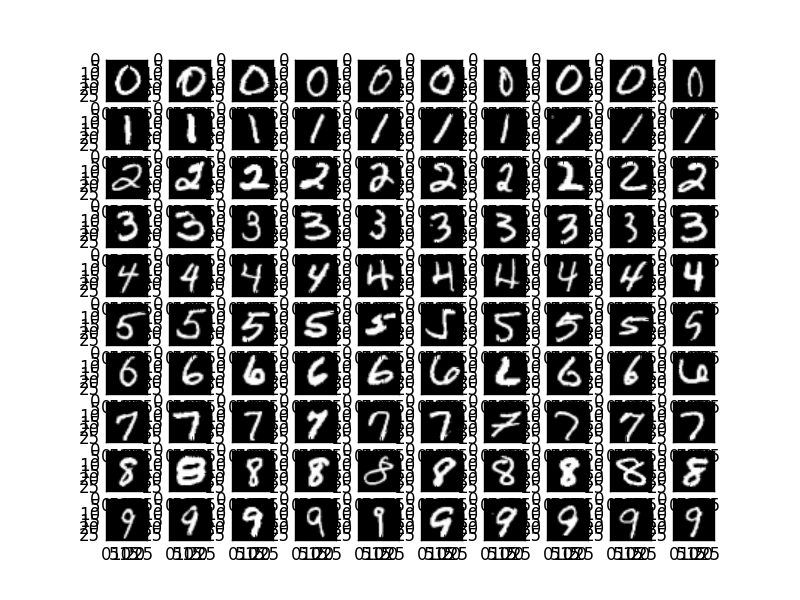
\includegraphics[scale=0.8]{part1.png}
	\caption*{10 images of digits from 0 to 9}
\end{figure*}

\clearpage

\section*{Part 2}

\paragraph{Question}
Implement a function that computes the network below.
\begin{figure*}[h]
	\centering
	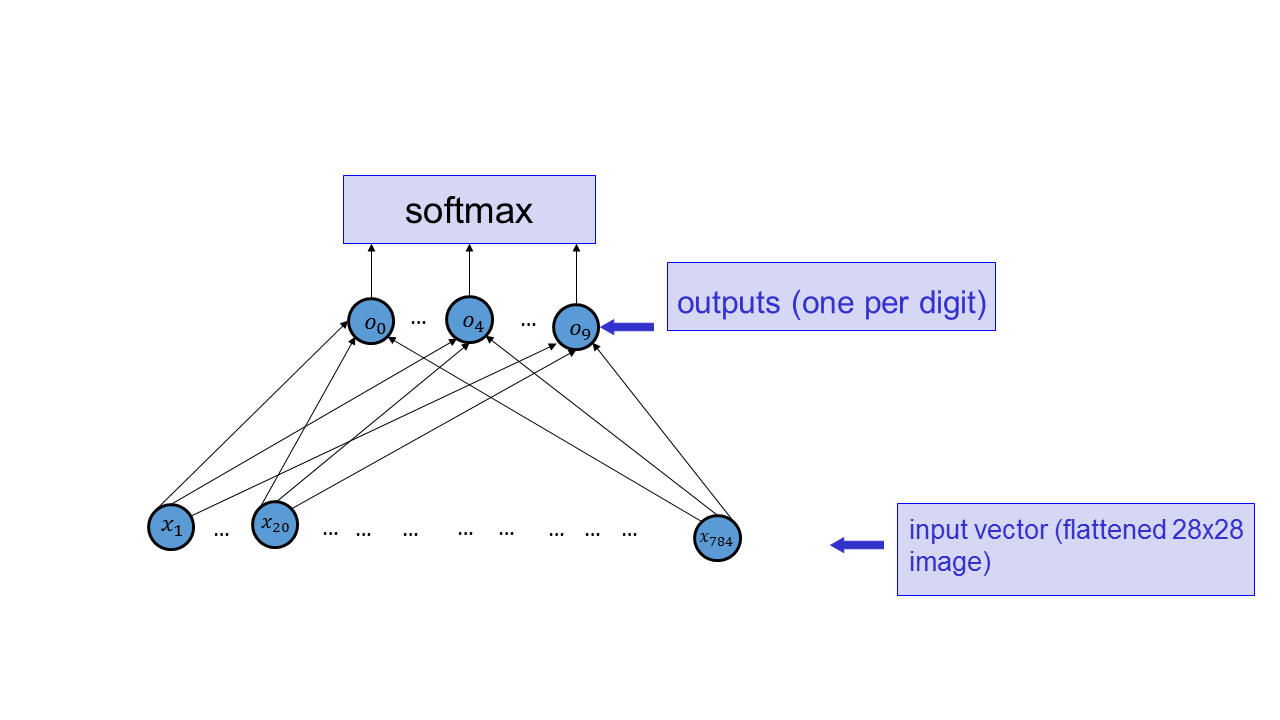
\includegraphics[scale=0.5]{logreg.png}
\end{figure*}
The $o$'s here should simply be linear combinations of the $x$'s (that is, the activation function in the output layer is the identity). Supecifically, use $o_i = \sum_{j}w_{ji}x_j+b_i$. Include the listing of your implementation in your report for this Part.

\paragraph{Answer}
Please see the source code of the function below:

\begin{lstlisting}[language=Python]
def softmax(y):
    '''Return the output of the softmax function for the matrix of output y. y
    is an NxM matrix where N is the number of outputs for a single case, and M
    is the number of cases'''
    return exp(y)/tile(sum(exp(y),0), (len(y),1))


def lin_combin(w, b, x):
    o = (dot(w.T, x) + b)
    return softmax(o)
\end{lstlisting}


\clearpage

\section*{Part 3}
We would like to use the sum of the negative log-probabilities of all the training cases as the cost function.

\subsection*{Part 3(a)}
\paragraph{Question}
Compute the gradient of the cost function with respect to the weight $w_{ij}$. Justify every step. You may refer to Slide 7 of the One-Hot Encoding lecture , but note that you need to justify every step there, and that your cost function is the sum over all the training examples.

\paragraph{Answer}
When sample size is one, we could calculate $\frac{\partial p_j}{\partial o_i}$ in two cases:
\begin{enumerate}
\item If $j = i$,
\begin{align*}
\frac{\partial p_i}{\partial o_i} &= \frac{e^{o_i}}{\sum_{k}e^{o_k}} - \frac{e^{o_i}}{\sum_{k}e^{o_k}} \cdot \frac{e^{o_i}}{\sum_{k}e^{o_k}}\\
&= p_i(1 - p_i)
\end{align*}
\item If $j \neq i$,
\begin{align*}
\frac{\partial p_j}{\partial o_i} &= -\frac{e^{o_j}}{\sum_{k}e^{o_k}} \cdot \frac{e^{o_i}}{\sum_{k}e^{o_k}}\\
&= -p_jp_i
\end{align*}
\end{enumerate}
In summary,
\begin{equation}
    \frac{\partial p_j}{\partial o_i} =
    \begin{cases*}
      p_i(1 - p_i) &, if $j = i$ \\
      -p_jp_i &, if $j \neq i$
    \end{cases*}
\end{equation}
\[\frac{\partial C}{\partial p_j} = -\frac{y_j}{p_j}\]
\begin{align*}
\frac{\partial C}{\partial o_{i}} &= \sum_{j}\frac{\partial C}{\partial p_j} \frac{\partial p_j}{\partial o_i}\\
&= \sum_{j, j \neq i}\frac{\partial C}{\partial p_j} \frac{\partial p_j}{\partial o_i} + \frac{\partial C}{\partial p_i} \frac{\partial p_i}{\partial o_i}\\
&= \sum_{j, j \neq i}(-\frac{y_j}{p_j}) \cdot (-p_jp_i) - \frac{y_i}{p_i} \cdot p_i(1 - p_i)\\
&= \sum_{j, j \neq i}y_jp_i - y_i + yip_i\\
&= \sum_{j}y_jp_i - y_i\\
\end{align*}
Because $\sum_{j}y_j = 1$, $\sum_{j}y_jp_i = p_i$. Then,
\begin{align*}
\frac{\partial C}{\partial o_{i}} &= p_i - y_i
\end{align*}
For the following equation, let $j$ refers to the input size (number of $x$ per sample) and $i$ refers to the output size (number of $o$ per sample), and $k$ refers to the training set size (number of samples).\\
\\
$X$ is the input matrix with dimension $n \times m$, where $n$ is the number $x$ (related to $j$) and $m$ is the sample size (related to $k$). $P$ is the calculated result matrix after using softmax with dimension $d \times m$, where $d$ is the output size (number of outputs per sample, related to $i$). $Y$ is the expected output with the same dimension as $P$.
\[\frac{\partial C}{\partial o_{ik}} = p_{ik} - y_{ik}\]
\begin{align*}
\frac{\partial o_{ik}}{\partial w_{ij}} &= \frac{\partial}{\partial w_{ij}}(w_{i1}x_{1k}+\dots+w_{ij}x_{jk}+\dots+w_{in}x_{nk}+b_{ik})\\
&=x_{jk}
\end{align*}
\begin{align*}
\frac{\partial C}{\partial w_{ij}} &= \sum_{k}\frac{\partial C}{\partial o_{ik}} \cdot \frac{\partial o_{ik}}{\partial w_{ij}}\\
&= \sum_{k}x_{jk}(p_{ik} - y_{ik})\\
&= X(P - Y)^T
\end{align*}
\subsection*{Part 3(b)}
\paragraph{Question}
Write vectorized code that computes the gradient with respect to the cost function. Check that the gradient was computed correctly by approximating the gradient at several coordinates using finite differences. Include the code for computing the gradient in vectorized form in your report.

\paragraph{Answer}
\begin{lstlisting}[language=Python]
def part3b(M):
    """Test gradient for part 3b."""
    
    x1 = M["train8"][0]
    x2 = M["train8"][1]
    x = vstack((x1, x2)).T
    y = array([[1, 0, 0, 0, 0, 0, 0, 0, 0, 0], [1, 0, 0, 0, 0, 0, 0, 0, 0, 0]]).T
    w = zeros((x.shape[0], 10))
    b = zeros((10, 2))
    test_gradient(x, y, b, w)


def test_gradient(x, y, b, w):
    """
    Compare the result of my gradient function NLL_gradient and the gradient get 
    from finite differences method. Test three times on different w_ij.
    """
    
    j_list = [5, 8, 8]
    i_list = [300, 601, 600]
    
    h = 10e-5
    
    for k in range(0, 3):
        i = i_list[k]
        j = j_list[k]
        g_finite = finite_diff_gradient(x, y, w, b, i, j, h)
        g_mine = NLL_gradient(x, y, w, b)[i, j]
        diff = abs(g_mine - g_finite)
        print("Test "+str(k)+":")
        print("gradient_finite_differences = "+str(g_finite))
        print("gradient_my_function = "+str(g_mine))
        print("difference = "+str(diff))
        print("-------------------------------")    


def finite_diff_gradient(x, y, w, b, i, j, h):
    """
    Use finite difference to calculate the gradient on w_ij with h.
    x: input
    y: expected output
    w: weight
    b: bias
    """
    
    c = NLL(x, y, w, b) 
    new_w = w
    new_w[i, j] += h
    new_c = NLL(x, y, new_w, b) 
    return (new_c - c)/h


def NLL(x, y, w, b):
    p = lin_combin(w, b, x)
    return -sum(y*log(p)) 
    
    
def NLL_gradient(x, y, w, b):
    p = lin_combin(w, b, x)
    return dot(x, (p - y).T)
\end{lstlisting}

\clearpage

\section*{Part 4}
\paragraph{Question}
Train the neural network you constructed. Plot the learning curves. Display the weights going into each of the output units. Describe the details of your optimization procedure.

\paragraph{Answer}
Please see the figures below.
\begin{figure*}[h]
	\centering
	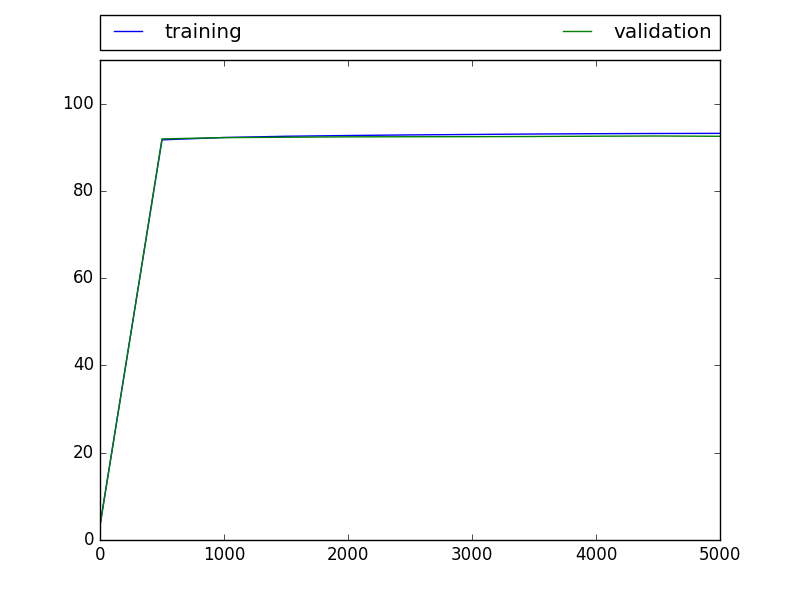
\includegraphics[scale=0.8]{part4.png}
	\caption*{Learning Curve}
\end{figure*}

\begin{figure*}[h]
	\centering
	\begin{subfigure}[h]{0.08\textwidth}
	\centering
	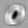
\includegraphics[scale=1]{w0.jpg}
	\caption*{w0}
	\end{subfigure}
	\begin{subfigure}[h]{0.08\textwidth}
	\centering
	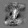
\includegraphics[scale=1]{w1.jpg}
	\caption*{w1}
	\end{subfigure}
	\begin{subfigure}[h]{0.08\textwidth}
	\centering
	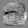
\includegraphics[scale=1]{w2.jpg}
	\caption*{w2}
	\end{subfigure}
	\begin{subfigure}[h]{0.08\textwidth}
	\centering
	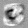
\includegraphics[scale=1]{w3.jpg}
	\caption*{w3}
	\end{subfigure}
	\begin{subfigure}[h]{0.08\textwidth}
	\centering
	
\includegraphics[scale=1]{w4.jpg}
	\caption*{w4}
	\end{subfigure}
	\begin{subfigure}[h]{0.08\textwidth}
	\centering
	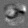
\includegraphics[scale=1]{w5.jpg}
	\caption*{w5}
	\end{subfigure}
	\begin{subfigure}[h]{0.08\textwidth}
	\centering
	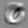
\includegraphics[scale=1]{w6.jpg}
	\caption*{w6}
	\end{subfigure}
	\begin{subfigure}[h]{0.08\textwidth}
	\centering
	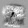
\includegraphics[scale=1]{w7.jpg}
	\caption*{w7}
	\end{subfigure}
	\begin{subfigure}[h]{0.08\textwidth}
	\centering
	
\includegraphics[scale=1]{w8.jpg}
	\caption*{w8}
	\end{subfigure}
	\begin{subfigure}[h]{0.08\textwidth}
	\centering
	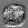
\includegraphics[scale=1]{w9.jpg}
	\caption*{w9}
	\end{subfigure}
\caption*{Weights corresponding to the 10 digits at 500 iterations}

We used gradient descent to train our network. Using the cost function and its gradient we got from previous parts, we ran gradient descent on both the weights and bias. We set the maximum number of iterations to 10000, EPS to $10^{-10}$, and we tested several times to get the alpha 0.00001.
\end{figure*}

\clearpage

\section*{Part 5}
\paragraph{Question}
The advantage of using multinomial logistic regression (i.e., the network you constructed here) over using linear regression as in Project 1 is that the cost function isn’t overly large when the actual outputs are very far away from the target outputs. That causes the network to not adjust the weights too much because of a single training case that causes the outputs to be very large. You should come up with a dataset where the performance on the test set is better when you use multinomial logistic regression. Do this by generating training and test sets similarly to how we did it in lecture . Show that the performance using multinomial logistic regression (on the test set) is substantially better. Explain what you did and include code to clarify your point. Clearly explain why your experiment illustrates your point.

\paragraph{Answer}
The dataset we have for training is as below.
\begin{figure*}[h]
	\centering
	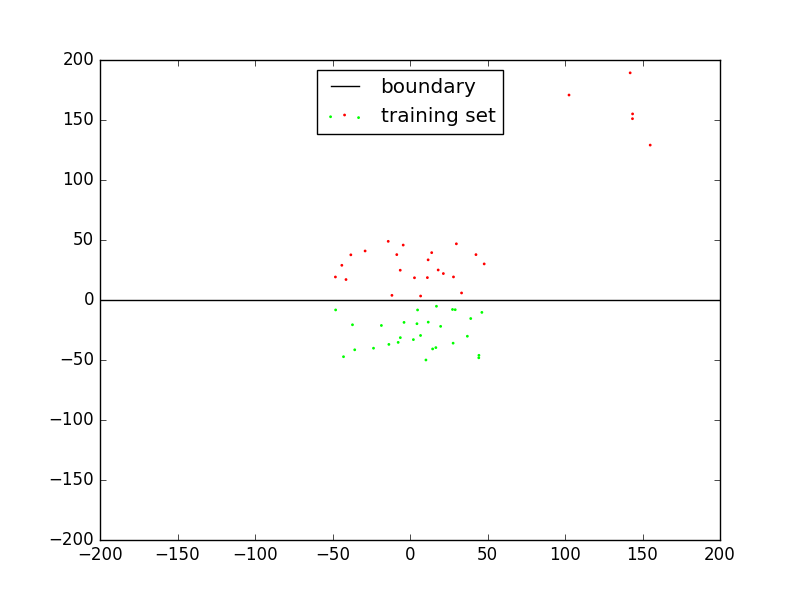
\includegraphics[scale=0.8]{part5_training_data.png}
	\caption*{Training Set}
\end{figure*}
We generated 50 generate samples in range $[-100, 100]$, and 5 outliers in range[100, 200] for both $x1$ and $x2$ (a sampe is $(x1, x2)$). The samples are classified into 2 classes. The samples above x-axis are classifies as Class 1 (the red points in graph), and others are classified as Class 2 (the green points in graph).\\
Since the output of logistic regression in within range of $(0, 1)$ and the output of linear regression is not limited, linear regression could not deal with outliers in data as good as logistic regression. In order to keep the cost small, my initial alpha of gradient descent for linear regression is $10^{-6}$, which is much smaller than my initial alpha for logistic regression (that is $10^{-3}$). The learning curve of linear regression and logistic regression on the dataset over iterations is shown below.
\begin{figure*}[h]
	\centering
	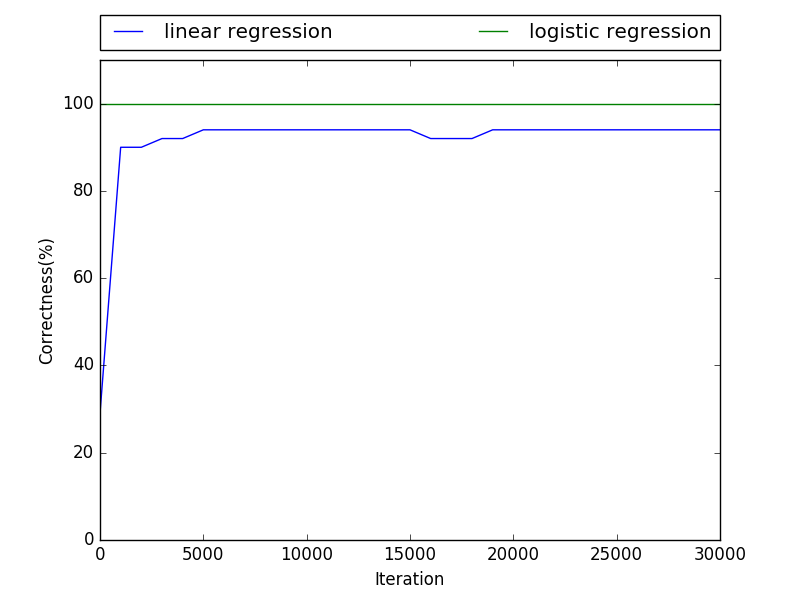
\includegraphics[scale=0.8]{part5_learning_curve.png}
	\caption*{Learning Curve of Linear Regression and Logistic Regression on Dataset}
\end{figure*}
From the figure we could see that logistic Regression gets to the minimum cost much faster than linear regression, and have better performance on training at the end.\\
The test data we have is shown below: 
\begin{figure*}[h]
	\centering
	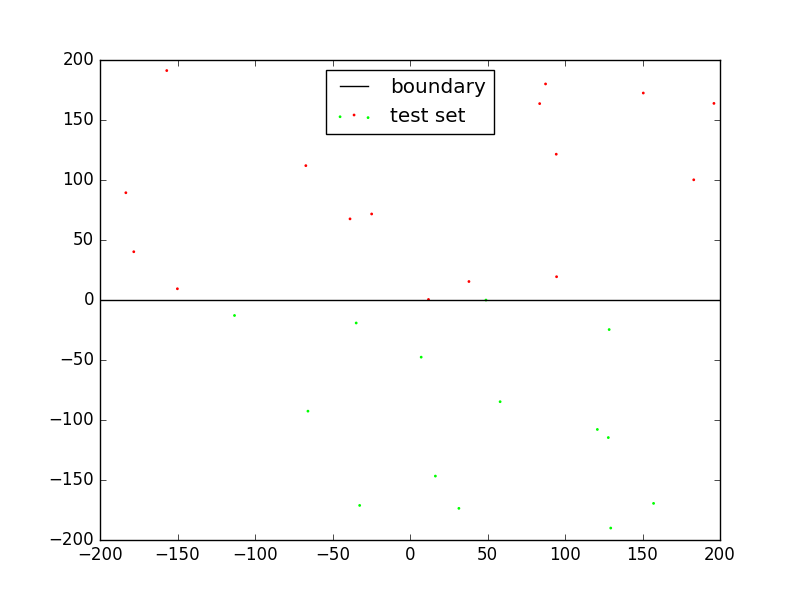
\includegraphics[scale=0.8]{part5_test_data.png}
	\caption*{Test Set}
\end{figure*}
The performance of linear regression is 83\% while the performance of logistic regression is 96\%.
\clearpage

\section*{Part 6}
\paragraph{Question}
Backpropagation can be seen as a way to speed up the computation of the gradient. For a network with $N$ layers each of which contains $K$ neurons, determine how much faster is (fully-vectorized) Backpropagation compared to computing the gradient with respect to each weight individually. Assume that all the layers are fully-connected. Show your work. Make any reasonable assumptions (e.g., about how fast matrix multiplication can be peformed), and state what assumptions you are making.

\paragraph{Answer}

Notation:
\begin{itemize}
\item $h_{iq}$ - $q$\textsuperscript{th} nequron in layer $i$
\item $w^{i,p,q}$ - weight from $p$\textsuperscript{th} neuron in layer $i-1$ to $q$\textsuperscript{th} neuron in layer $i$
\item Assume for each neuron $h_{iq}$, $h_{iq} = \sum_p w^{i, p, q}h_{i-1, p}+b_{i, q}$
\item Assume the model is the same model as earlier parts, so $o_i$s $\rightarrow$ softmax $\rightarrow$ $p_i$s $\rightarrow$ NLL
\item Assume the model is for one sample in the training set
\end{itemize}
\begin{enumerate}
\item 
\[\frac{\partial C}{\partial w_{n, p, q}} = \frac{\partial C}{\partial o_q} \cdot \frac{\partial o_q}{\partial w^{n, p, q}} = (p_q \cdot y_q)h_{n-1, p}\]
\[\nabla_nC = (H_{n-1})^T(P-Y)\]
where $H$, $P$, and $Y$ are $k \times 1$ vectors.
\item 
\[\frac{\partial C}{\partial h_{n-1, q}} = \sum_i \frac{\partial C}{\partial o_i} \cdot \frac{\partial o_i}{\partial h_{n-1, q}} = \sum_i \frac{\partial C}{\partial o_i} \cdot w^{n, q, i}\]
Then, 
\[\frac{\partial C}{\partial h_{n-1}} = W^n \cdot \frac{\partial C}{\partial O}\]
where $W^n$ is a $k \times k$ matrix and $\frac{\partial C}{\partial O}$ is a $k \times 1$ vector.
\item \[\frac{\partial C}{\partial w^{n-1, p, q}} = \frac{\partial C}{\partial h_{n-1, q}} \cdot \frac{\partial h_{n-1, q}}{\partial w^{n-1, p, q}} = \frac{\partial C}{\partial h_{n-1, q}} \cdot h_{n-2, p}\]
\[\nabla_{n-1}C = (\frac{\partial C}{\partial H_{n-1}})^T \cdot H_{n-2}\]
where $\frac{\partial C}{\partial H_{n-1}}$ and $H_{n-2}$ are $k \times 1$ vectors.
\item \[\frac{\partial C}{\partial h_{n-2}, q} = \sum_i \frac{\partial C}{\partial h_{n-1, i}} \cdot \frac{\partial h_{n-1, i}}{\partial h_{n-2, q}} = \sum_i \frac{\partial C}{\partial h_{n-1, i}} \cdot w^{n-1, q, i}\]
\[\nabla_{n-2} C = (\frac{\partial C}{\partial H_{n-1}})^T \cdot H_{n-3}\]
\end{enumerate}
In conclusion, for layer $i$:
\[\frac{\partial C}{\partial H_i} =  W^{i+1} \cdot \frac{\partial C}{\partial H_{i+1}}\]
which have $k^2$ multiplication.
\[\nabla_i C = \frac{\partial C}{\partial H_i} \cdot H_{i-1}\]
which have $k$ multiplication.
So for $n-1$ layers, we have $k^2(n-1)$ multiplications, and $n$ gradient calculation takes $kn$ multiplications. The runtime for backpropagation is polynomial. If we don't use backpropagation and any storage method, for layer $i$, we need to recalculate layer the derivative at layer $i+1$, the runtime is exponential. Therefore, backpropagation speed up the computation of the gradient.

\clearpage

\section*{Part 7}
\paragraph{Question}
I am providing the TensorFlow code for training a single-hidden-layer fully-connected network here. The training is done using mini-batches. Modify the code to classify faces of the 6 actors in Project 1. Use a fully-connected neural network with a single hidden layer. In your report, include the learning curve for the test, training, and validation sets, and the final performance classification on the test set. Include a text description of your system. In particular, describe how you preprocessed the input and initialized the weights, what activation function you used, and what the exact architecture of the network that you selected was. Experiment with different settings to produce the best performance, and report what you did to obtain the best performance.\\

Use 30 images per actor in the test set.\\

Unlike in Project 1, you must remove non-faces from your dataset. Use the SHA-256 hashes to remove bad images. You may additionally hardcode the indices of the images that you’d like to remove.\\

\paragraph{Answer}
\begin{figure*}[h]
	\centering
	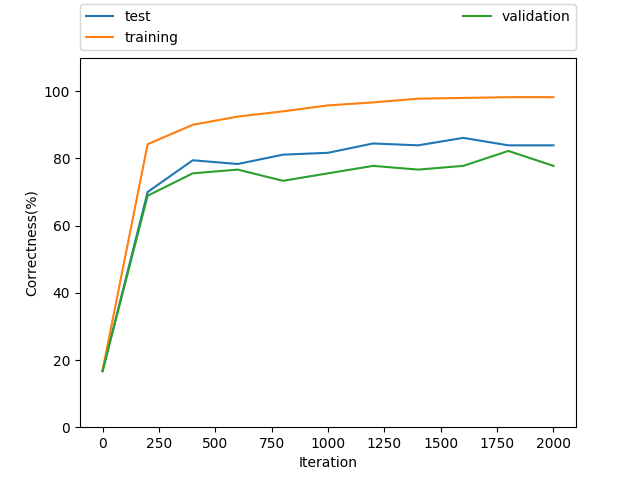
\includegraphics[scale=0.8]{part7.png}
	\caption*{Part 7 Learning Curve}
\end{figure*}

The final performance on test set is 87\%.\\
Before starting building the network, we need to first preprocess the images. Similar to Project 1, we downloaded the images using actors.txt. Then the images are cropped, greyscaled, and saved in the cropped folder. However we also check the hash of each image (indication of bad image). If it doesn't match with the hash code provided in actors.txt, we will not save it in the cropped folder either.
Afterwards, we need to split the dataset into 3 - training, test, and validation. However, due to the hash code limitation, there are less images for each actors compare to Project 1. In the end we decided to split the dataset this way:
\begin {itemize}
	\item 30 images per actor in the test set. (as requested)
	\item 75 images per actor in the training set. We tried to make the training set as large as possible while maintaining a reasonable size for the validation set.
	\item 15 images per actor in the validation. The size of validation is usually smaller than the test set and training set. However at the same time we didn't want to make the validation set to be too small. Therefore we made it 15 images.
\end {itemize}
As for the structure, we used a very similar architecture to the started code provided. In the structure, we have:
\begin {itemize}
	\item Input layer of size 1024
	\item A single layer of 100 hidden units. Each hidden unit is fully connected to the input layer. The activation of the hidden units is $tanh$, so that the weights can be pulled towards different direction when training the model.
	\item A output layer consist of 6 units that are all fully connected to the 100 hidden units. The activation of the output layer is just itself (matrix multiplication).
	\item The output layer will be passed into a softmax. Then the output of softmax will be used to calculate the Negative Log Loss cost of the model.
	\item We also randomly select a mini-batch at each training iteration to avoid local minima.
	\item We use the $Adam Optimizer$ for training. It is a variation of gradient descent.
\end {itemize}
For the weights, we randomly initiated it to small random numbers to break the symmetry.
As for parameters (eg. mini-batch size, number of hidden units, $\alpha$ etc) and the structure of network, we obtained them through trial and error. We experiemented with different setting, and decided each parameter based on the validation performance.

\clearpage

\section*{Part 8}
\paragraph{Question}
You are not required to use regularization in Part 7 (although that would produce nicer weight visualization). Find a scenario where using regularization is necessary in the context of face classification, and find the best regularization parameter $\lambda$.

\paragraph{Answer}
Regularization prevents overfitting, so we tried to come up a dataset that could have overfitting. We have a training set of all 6 actors from part 7 but each actor only has 1 image. The validation set contains 20 images per actor, and the test set contains 100 images per actor. Without regularization, the performance on training set after 8000 iterations is 100\%, while test set performance is 30\%. With regularization where $\lambda = 10^{-9}$, the performance of test set increased to 33\%. The difference equals $\frac{75}{\sqrt{600}}$ where 600 is the test set size. Therefore, regularization is necessary in the context of face classification.

\end{document}